% -*- coding: utf-8 -*-
%-------------------------designed by zcf--------------
\documentclass[UTF8,a4paper,10pt]{ctexart}
\usepackage[left=3.17cm, right=3.17cm, top=2.74cm, bottom=2.74cm]{geometry}
\usepackage{amsmath}
\usepackage{graphicx,subfig}
\usepackage{float}
\usepackage{cite}
\usepackage{caption}
\usepackage{enumerate}
\usepackage{booktabs} %表格
\usepackage{multirow}
\newcommand{\tabincell}[2]{\begin{tabular}{@{}#1@{}}#2\end{tabular}}  %表格强制换行
%-------------------------字体设置--------------
\usepackage{times} 
\newcommand{\yihao}{\fontsize{26pt}{36pt}\selectfont}           % 一号, 1.4 倍行距
\newcommand{\erhao}{\fontsize{22pt}{28pt}\selectfont}          % 二号, 1.25倍行距
\newcommand{\xiaoer}{\fontsize{18pt}{18pt}\selectfont}          % 小二, 单倍行距
\newcommand{\sanhao}{\fontsize{16pt}{24pt}\selectfont}  %三号字
\newcommand{\xiaosan}{\fontsize{15pt}{22pt}\selectfont}        % 小三, 1.5倍行距
\newcommand{\sihao}{\fontsize{14pt}{21pt}\selectfont}            % 四号, 1.5 倍行距
\newcommand{\banxiaosi}{\fontsize{13pt}{19.5pt}\selectfont}    % 半小四, 1.5倍行距
\newcommand{\xiaosi}{\fontsize{12pt}{18pt}\selectfont}            % 小四, 1.5倍行距
\newcommand{\dawuhao}{\fontsize{11pt}{11pt}\selectfont}       % 大五号, 单倍行距
\newcommand{\wuhao}{\fontsize{10.5pt}{15.75pt}\selectfont}    % 五号, 单倍行距
%-------------------------章节名----------------
\usepackage{ctexcap} 
\CTEXsetup[name={,、},number={ \chinese{section}}]{section}
\CTEXsetup[name={(,)},number={\chinese{subsection}}]{subsection}
\CTEXsetup[name={,.},number={\arabic{subsubsection}}]{subsubsection}
%-------------------------页眉页脚--------------
\usepackage{fancyhdr}
\pagestyle{fancy}
\lhead{\kaishu \leftmark}
% \chead{}
\rhead{\kaishu 编译原理作业报告}%加粗\bfseries 
\lfoot{}
\cfoot{\thepage}
\rfoot{}
\renewcommand{\headrulewidth}{0.1pt}  
\renewcommand{\footrulewidth}{0pt}%去掉横线
\newcommand{\HRule}{\rule{\linewidth}{0.5mm}}%标题横线
\newcommand{\HRulegrossa}{\rule{\linewidth}{1.2mm}}
%-----------------------伪代码------------------
\usepackage{algorithm}  
\usepackage{algorithmicx}  
\usepackage{algpseudocode}  
\floatname{algorithm}{Algorithm}  
\renewcommand{\algorithmicrequire}{\textbf{Input:}}  
\renewcommand{\algorithmicensure}{\textbf{Output:}} 
\usepackage{lipsum}  
\makeatletter
\newenvironment{breakablealgorithm}
  {% \begin{breakablealgorithm}
  \begin{center}
     \refstepcounter{algorithm}% New algorithm
     \hrule height.8pt depth0pt \kern2pt% \@fs@pre for \@fs@ruled
     \renewcommand{\caption}[2][\relax]{% Make a new \caption
      {\raggedright\textbf{\ALG@name~\thealgorithm} ##2\par}%
      \ifx\relax##1\relax % #1 is \relax
         \addcontentsline{loa}{algorithm}{\protect\numberline{\thealgorithm}##2}%
      \else % #1 is not \relax
         \addcontentsline{loa}{algorithm}{\protect\numberline{\thealgorithm}##1}%
      \fi
      \kern2pt\hrule\kern2pt
     }
  }{% \end{breakablealgorithm}
     \kern2pt\hrule\relax% \@fs@post for \@fs@ruled
  \end{center}
  }
\makeatother
%------------------------代码-------------------
\usepackage{xcolor} 
\usepackage{listings} 
\usepackage{fontspec}
\newfontfamily\menlo{Menlo}
\setmonofont[Mapping={}]{Monaco} 
\definecolor{mygreen}{rgb}{0,0.6,0}
\definecolor{mygray}{rgb}{0.5,0.5,0.5}
\definecolor{mymauve}{rgb}{0.58,0,0.82}
\lstset{ %
backgroundcolor=\color{white},   % choose the background color
basicstyle=\footnotesize\ttfamily,        % size of fonts used for the code
columns=fullflexible,
breaklines=true,                 % automatic line breaking only at whitespace
captionpos=b,                    % sets the caption-position to bottom
tabsize=4,
commentstyle=\color{mygreen},    % comment style
escapeinside={\%*}{*)},          % if you want to add LaTeX within your code
keywordstyle=\color{blue},       % keyword style
stringstyle=\color{mymauve}\ttfamily,     % string literal style
frame=single,
rulesepcolor=\color{red!20!green!20!blue!20},
numbers=left,
 numberstyle=\tiny\menlo
% identifierstyle=\color{red},
% language=c++,
}
%------------超链接----------
\usepackage[colorlinks,linkcolor=black,anchorcolor=blue]{hyperref}
%------------------------TODO-------------------
\usepackage{enumitem,amssymb}
\newlist{todolist}{itemize}{2}
\setlist[todolist]{label=$\square$}
% for check symbol 
\usepackage{pifont}
\newcommand{\cmark}{\ding{51}}%
\newcommand{\xmark}{\ding{55}}%
\newcommand{\done}{\rlap{$\square$}{\raisebox{2pt}{\large\hspace{1pt}\cmark}}\hspace{-2.5pt}}
\newcommand{\wontfix}{\rlap{$\square$}{\large\hspace{1pt}\xmark}}
%------------------------水印-------------------
\usepackage{tikz}
\usepackage{xcolor}
\usepackage{eso-pic}

\newcommand{\watermark}[3]{\AddToShipoutPictureBG{
\parbox[b][\paperheight]{\paperwidth}{
\vfill%
\centering%
\tikz[remember picture, overlay]%
  \node [rotate = #1, scale = #2] at (current page.center)%
    {\textcolor{gray!80!cyan!30!magenta!30}{#3}};
\vfill}}}



%———————————————————————————————————————————正文———————————————————————————————————————————————
%----------------------------------------------
\begin{document}
\begin{titlepage}
    \begin{center}
    
\includegraphics[width=0.8\textwidth]{NKU.png}\\[1cm]    
    \textsc{\Huge \kaishu{\textbf{南\ \ \ \ \ \ 开\ \ \ \ \ \ 大\ \ \ \ \ \ 学}} }\\[0.9cm]
    \textsc{\huge \kaishu{\textbf{计\ \ 算\ \ 机\ \ 学\ \ 院}}}\\[0.5cm]
    \textsc{\Large \textbf{计算机系统设计}}\\[0.8cm]
    \HRule \\[0.9cm]
    { \LARGE \bfseries PA实验四报告}\\[0.4cm]
    \HRule \\[2.0cm]
    \centering
    \textsc{\LARGE \kaishu{朱浩泽\ 1911530}}\\[0.5cm]
    \textsc{\LARGE \kaishu{年级\ :\ 2019级}}\\[0.5cm]
    \textsc{\LARGE \kaishu{专业\ :\ 计算机科学与技术}}\\[0.5cm]
    \textsc{\LARGE \kaishu{指导教师\ :\ 卢冶}}\\[0.5cm]
    \vfill
    {\Large \today}
    \end{center}
\end{titlepage}
% -------------摘------要--------------
\newpage
\thispagestyle{empty}
% ----------------------------------------------------------------
\tableofcontents
% ----------------------------------------------------------------
\newpage
\watermark{60}{10}{NKU}
\setcounter{page}{1}
\section{概述}
\subsection{实验目的}
\begin{itemize}
  \item 学习虚拟内存映射,并实现分页机制
  \item 学习上下文切换的基本原理并实现上下文切换、进程调度与分时多任务 
  \item 学习硬件中断并实现时钟中断
\end{itemize}
\subsection{实验内容}
\begin{itemize}
  \item 虚拟地址空间的作用,实现分页机制,并让用户程序运行在分页机制上
  \item 实现内核自陷、上下文切换与分时多任务
  \item 解决阶段二分时多任务的隐藏bug:改为使用时钟中断来进行进程调度
  \item 实现当前运行游戏的切换,使不同的游戏与hello程序分时运行
\end{itemize}

\section{阶段一: 实现分页机制}
\subsection{基础结构}
首先修改寄存器结构体,在 nemu/include/cpu/reg.h当中,添加CR0和CR3两个控制寄存器:
\begin{lstlisting}[language=C++]
struct IDTR
  {
    /* data */
    uint32_t base;
    uint16_t limit; 
  } idtr;
  
  rtlreg_t cs;
  rtlreg_t es; // 配x64
  rtlreg_t ds;
  uint32_t CR0;
  uint32_t CR3;
  bool INTR;
} CPU_state;
\end{lstlisting}
然后在nemu/src/monitor/monitor.c的resart函数中初始化CR0的值
\begin{lstlisting}[language = C++]
static inline void restart() {
  /* Set the initial instruction pointer. */
  cpu.eip = ENTRY_START;
  cpu.cs = 8;
  cpu.CR0 = 0x60000011;
  unsigned int origin = 2;
  memcpy(&cpu.eflags, &origin, sizeof(cpu.eflags));

#ifdef DIFF_TEST
  init_qemu_reg();
#endif
}
\end{lstlisting}
打开 HAS\_PTE 宏,让Nanos-lite 在初始化的时候首先调用 init\_mm()函数。在nanos-lite目录下make run,报错如下:
\begin{center}
  \includegraphics*[scale = 0.5]{img/1}
\end{center}

到目前这个阶段而言,init\_mm()函数的工作主要有两方面,一是将空闲物理页的首地址设置为堆区首地址;二是调用\_pte\_init()函数,填写内核的页目录和页表,设置控制寄存器,开启分页机制。\\ 
于是,我们首先需要实现新的指令函数,来完成对两个控制寄存器的操作。相关代码在 nemu/include/cpu/rtl.h中添加。\\ 
首先完成nemu/include/cpu/rtl.h中的rtl\_store\_cr(int r, const rtlreg\_t* src)函数,实现对控制信息的存储,根据情况把参数保存到CR0寄存器或CR3寄存器当中。
\begin{lstlisting}[language = C++]
static inline rtl_store_cr(int r, const rtlreg_t* src) {
  switch (r)
  {
  case 0:
    cpu.CR0 = *src;
    return;
  case 3:
    cpu.CR3 = *src;
    return;
  default:
    assert(0);
  }
  return;
}
\end{lstlisting}

完成nemu/include/cpu/rtl.h中的rtl\_load\_cr(rtlreg\_t* dest, int r)函数,实现对控制信息的读取,根据情况把CR0或CR3寄存器当中存储的信息读取到dest参数中。

\begin{lstlisting}[language = C++]
static inline rtl_load_cr(rtlreg_t* dest, int r) {
  switch (r)
  {
  case 0:
    *dest = cpu.CR0;
    return;
    break;
  case 3:
    *dest = cpu.CR3;
    return;
  default:
    assert(0);
  }
  return;
}
\end{lstlisting}

然后完成init\_mm()函数遇到的指令,即CR3或CR0的mov操作。
在 nemu/src/cpu/decode/decode.c中实现译码函数,其中make\_DHelper(mov\_load\_cr)完成的是把控制寄存器中所存储的值进行加载读取的操作,make\_DHelper(mov\_load\_cr)完成的是把目标寄存器的值保存到控制寄存器的操作。
\begin{lstlisting}[language = C++]
make_DHelper(mov_load_cr) {
  decode_op_rm(eip, id_dest, false, id_src, false);
  rtl_load_cr(&id_src -> val, id_src -> reg);
#ifdef DEBUG
  snprintf(id_src -> str, 5, "%%cr%d", id_dest -> reg);
#endif
}

make_DHelper(mov_store_cr) {
  decode_op_rm(eip, id_src, true, id_dest, false);
#ifdef DEBUG
  snprintf(id_src -> str, 5, "%%cr%d", id_dest -> reg);
#en
\end{lstlisting}


最后在nemu/src/cpu/exec/data-mov.c中添加实际的指令函数make\_EHelper(mov\_store\_cr),来完成控制寄存器的store操作。
\begin{lstlisting}[language = C++]
make_EHelper(mov_store_cr) {
  rtl_store_cr(id_dest -> reg, &id_src -> val);
  print_asm_template2(mov);
}
\end{lstlisting}


到此,分页机制的数据结构基础部分我们已经基本完成。通过设置断点,我们可以看到如下内容:
\begin{center}
  \includegraphics*[scale = 0.25]{img/2}
  \includegraphics*[scale = 0.25]{img/3}
\end{center}

\subsection{虚拟地址的访问的转换}
接下来需要对nemu/src/memory/memory.c中的 vaddr\_read()和 vaddr\_write()函数作少量修改、实现page\_translate()函数,使得所有虚拟地址的访问都需要经过分页地址的转换。


首先,在nemu/src/memory/memory.c中添加我们需要的宏定义。
\begin{lstlisting}[language = C++]
#define PTXSHFT 12 //线性地址偏移量
#define PDXSHFT 22 //线性地址偏移量 

#define PTE_ADDR(pte) ((uint32_t)(pte) & ~0xfff)
#define PDX(va) (((uint32_t)(va) >> PDXSHFT) & 0x3ff)
#define PTX(va) (((uint32_t)(va) >> PTXSHFT) & 0x3ff)
#define OFF(va) ((uint32_t)(va) & 0xfff)
\end{lstlisting}
vaddr\_read(vaddr\_t addr, int len)函数实现了读地址时的虚拟地址转换。
\begin{lstlisting}[language = C++]
uint32_t vaddr_read(vaddr_t addr, int len) {
  if(PTE_ADDR(addr) != PTE_ADDR(addr + len -1)) {
    // printf("error: the data pass two pages:addr=0x%x, len=%d!\n", addr, len);
    assert(0);
  }
  else {
    paddr_t paddr = page_translate(addr, false);
    return paddr_read(paddr, len);
  }
  // return paddr_read(addr, len);
}
\end{lstlisting}
vaddr\_write(vaddr\_t addr, int len)函数实现了写地址时的虚拟地址转换。
\begin{lstlisting}[language = C++]
  void vaddr_write(vaddr_t addr, int len, uint32_t data) {
  if(PTE_ADDR(addr) != PTE_ADDR(addr+len-1)) {
    // printf("error: the data pass two pages:addr=0x%x, len=%d!\n", addr, len);
    assert(0);
    }
  }
  else {
    paddr_t paddr = page_translate(addr, true);
    paddr_write(paddr, len, data);
  }
  // paddr_write(addr, len, data);
}
\end{lstlisting}
其中,如果存在跨页读写的现象,暂且不做处理,直接结束程序。
这里的page\_translate()函数是实验指导书要求实现的页面地址转换函数,接下来我们就需要对这个函数进行编写。
\begin{lstlisting}[language = C++]
paddr_t page_translate(vaddr_t addr, bool iswrite) {
  CR0 cr0 = (CR0)cpu.CR0;
  if(cr0.paging && cr0.protect_enable) {
    CR3 crs = (CR3)cpu.CR3;

    PDE *pgdirs = (PDE*)PTE_ADDR(crs.val);
    PDE pde = (PDE)paddr_read((uint32_t)(pgdirs + PDX(addr)), 4);

    PTE *ptable = (PTE*)PTE_ADDR(pde.val);
    PTE pte = (PTE)paddr_read((uint32_t)(ptable + PTX(addr)), 4);
    //printf("hhahah%x, jhhh%x\n", pte.present, addr);
    Assert(pte.present, "addr=0x%x", addr);

    pde.accessed=1;
    pte.accessed=1;
    if(iswrite) {
      pte.dirty=1;
    }
    paddr_t paddr = PTE_ADDR(pte.val) | OFF(addr);
    // printf("vaddr=0x%x, paddr=0x%x\n", addr, paddr);
    return paddr;
  }
	return addr;
}
\end{lstlisting}
在page\_translate(vaddr\_t addr, bool\ iswrite)函数当中,参数addr代表待处理页面的地址,iswrite是读或写的标志位,若需要进行的是读操作,该参数就被设置为false,若需要进行写操作,就被设置为true。\\
这个函数需要依次判断页目录、页表是否存在,并根据读写情况对页面进行脏位标记。如果页面不存在,需要呈现错误信息并结束程序。

运行程序,可以发现,这时候的虚拟地址和物理地址是相同的,我们的初步分页算法实现成功。

\begin{center}
  \includegraphics*[scale = 0.28]{img/4}
\end{center}
但这个算法只能在单页面内有效,如果出现了跨页的情况,就会按我们在vaddr\_read()和vaddr\_write()函数中所设定的一样,结束程序。
\begin{center}
  \includegraphics*[scale = 0.28]{img/5}
\end{center}
为了解决跨页问题,我们还需要进一步修改nemu/src/memory/memory.c中的这两个读写函数。
\begin{lstlisting}[language = C++]
uint32_t vaddr_read(vaddr_t addr, int len) {
  if(PTE_ADDR(addr) != PTE_ADDR(addr + len -1)) {
    // printf("error: the data pass two pages:addr=0x%x, len=%d!\n", addr, len);
    // assert(0);
    int num1 = 0x1000 - OFF(addr);
    int num2 = len - num1;
    paddr_t paddr1 = page_translate(addr, false);
    paddr_t paddr2 = page_translate(addr + num1, false);

    uint32_t low = paddr_read(paddr1, num1);
    uint32_t high = paddr_read(paddr2, num2);

    uint32_t result = high << (num1 * 8) | low;
    return result;
  }
  else {
    paddr_t paddr = page_translate(addr, false);
    return paddr_read(paddr, len);
  }
  // return paddr_read(addr, len);
}
\end{lstlisting}
如果出现了跨页的情况,就分高低页进行读取,用两个num局部变量记录高低页的字节数,paddr记录高低页对应物理地址,再进行整合读取。\\
跨页写入的情况和跨页读取类似。
\begin{lstlisting}[language = C++]
void vaddr_write(vaddr_t addr, int len, uint32_t data) {
  if(PTE_ADDR(addr) != PTE_ADDR(addr+len-1)) {
    // printf("error: the data pass two pages:addr=0x%x, len=%d!\n", addr, len);
    // assert(0);
    if(PTE_ADDR(addr) != PTE_ADDR(addr + len -1)) {
      int num1 = 0x1000-OFF(addr);
      int num2 = len -num1;
      paddr_t paddr1 = page_translate(addr, true);
      paddr_t paddr2 = page_translate(addr + num1, true);

      uint32_t low = data & (~0u >> ((4 - num1) << 3));
      uint32_t high = data >> ((4 - num2) << 3);

      paddr_write(paddr1, num1, low);
      paddr_write(paddr2, num2, high);
      return;
    }
  }
  else {
    paddr_t paddr = page_translate(addr, true);
    paddr_write(paddr, len, data);
  }
  // paddr_write(addr, len, data);
}
\end{lstlisting}
完善这两个函数之后,跨页问题就得到了解决,程序可以正确运行。
\begin{center}
  \includegraphics*[scale = 0.28]{img/7}
  \includegraphics*[scale = 0.32]{img/8}
\end{center}
\subsection{让用户程序运行在分页机制上}
实现了分页机制之后,我们回归到最初的目的:让用户程序能够分时运行。所以本阶段这部分内容需要将用户程序也运行在我们已经实现好的分页机制上。先按指导书修改navy¬-apps/Makefile.compile,把链接地址改成0x8048000:
\begin{lstlisting}
ifeq ($(LINK), dynamic)
  CFLAGS   += -fPIE
  CXXFLAGS += -fPIE
  LDFLAGS  += -fpie -shared
else
  LDFLAGS += -Ttext 0x8048000
endif
\end{lstlisting}
同时也相对应地修改nanos-lite/src/loader.c当中对DEFAULT\_ENTRY的宏定义:
\begin{lstlisting}[language = C++]
#define DEFAULT_ENTRY ((void *)0x8048000)
\end{lstlisting}
运行dummy报缺页错误,这是因为我们尚未实现页的分配和映射,所以运行会有问题。
\begin{center}
  \includegraphics*[scale = 0.28]{img/6}
\end{center}

于是,在nexus-am/am/arch/x86-nemu/src/pte.c当中实现\_map()函数。这个函数的具体功能是将虚拟地址空间 p 中的虚拟地址 va 映射到物理地址 pa,通过 p->ptr 可以获取页目录的基地址;如果映射过程中发现需要申请新的页,就调用palloc\_f()函数来完成。
\begin{lstlisting}[language = C++]
void _map(_Protect *p, void *va, void *pa) {
  if(OFF(va) || OFF(pa)) {
    // printf("page not aligned\n");
    return;
  }

  PDE *dir = (PDE*) p -> ptr;
	PTE *table = NULL;
	PDE *pde = dir + PDX(va);
	if(!(*pde & PTE_P)) {
		table = (PTE*) (palloc_f());
		*pde = (uintptr_t) table | PTE_P;
	}
	table = (PTE*) PTE_ADDR(*pde);
	PTE *pte = table + PTX(va);
	*pte = (uintptr_t) pa | PTE_P;
}
\end{lstlisting}
完成了页面的分配和映射,还需要让loader也按页加载。在nanos-lite/src/loader.c中对loader函数进行修改
\begin{lstlisting}[language = C++]
uintptr_t loader(_Protect *as, const char *filename) {
  // TODO();
  // ramdisk_read(DEFAULT_ENTRY, 0, RAMDISK_SIZE);
  int fd = fs_open(filename, 0, 0);
  Log("filename=%s,fd=%d",filename,fd);
  // fs_read(fd, DEFAULT_ENTRY, fs_filesz(fd));
  int size = fs_filesz(fd);
  int ppnum = size / PGSIZE;
  if(size % PGSIZE != 0) {
    ppnum++;
  }
  void *pa = NULL;
  void *va = DEFAULT_ENTRY;
  for(int i = 0; i < ppnum; i++) {
    pa = new_page();
    _map(as, va, pa);
    fs_read(fd, pa, PGSIZE);
    va += PGSIZE;
  }

  fs_close(fd);
  return (uintptr_t)DEFAULT_ENTRY;
}
\end{lstlisting}
此时dummy已经可以正确运行,但仙剑奇侠传还是有一些需要进一步实现和完善的地方。为了让仙剑奇侠传在分页机制上运行,我们需要完成堆内存的映射,实现nanos-lite/src/mm.c当中的mm\_brk()函数。在PA3的实现中,我们直接让这个函数返回0,表示用户程序的堆区大小修改总是成功。但实现分页之后,用户程序运行在虚拟地址空间之上,于是我们在这个函数中完成了把新申请的堆区映射到虚拟地址空间中的工作
\begin{lstlisting}[language = C++]
int mm_brk(uint32_t new_brk) {
  if(current -> cur_brk == 0) {
    current -> cur_brk = current -> max_brk = new_brk;
  }
  else {
    if(new_brk > current -> max_brk) {
      uint32_t first = PGROUNDUP(current -> max_brk);
      uint32_t end = PGROUNDDOWN(new_brk);
      if((new_brk & 0xfff) == 0) {
        end -= PGSIZE;
      }
      for(uint32_t va = first; va <= end; va += PGSIZE) {
        void *pa = new_page();
        _map(&(current -> as), (void*)va, pa);
      }
      current -> max_brk = new_brk;
    }
    current -> cur_brk = new_brk;
  }
  return 0;
}
\end{lstlisting}
修改nanos-lite/src/syscall.c中与之对应的sys\_brk()函数
\begin{lstlisting}[language = C++]
int sys_brk(int addr) {
  extern int mm_brk(uint32_t new_brk);
  return mm_brk(addr);
}
\end{lstlisting}
完成后,仙剑奇侠传已经可以正常运行,PA4第一阶段到此结束。
\begin{center}
  \includegraphics*[scale = 0.4]{img/8}
\end{center}

\section{阶段二: 上下文切换与调度}
在这一阶段,我们需要内核自陷、上下文切换,以最终实现程序的分时运行。
\subsection{内核自陷}
在真实的操作系统当中,程序通过自陷指令触发上下文切换,所以我们首先实现内核自陷。
第一,	在nanos-lite/src/main.c中开启内核自陷的功能:\_trap();我们约定内核自陷通过指令 int \$0x81触发,于是据此完成\_tarp()函数。调整nexus-am/am/arch/x86-nemu/src/asye.c中的\_trap()函数
\begin{lstlisting}[language = C++]
void _trap() {
  asm volatile("int $0x81");
}
\end{lstlisting}
然后,在nanos-lite/src/proc.c中的load\_prog函数注释代码如下:
\begin{lstlisting}[language = C++]
// TODO: remove the following three lines after you have implemented _umake()
// _switch(&pcb[i].as);
// current = &pcb[i];
// Log("run proc go to %x", entry);
// ((void (*)(void))entry)();
\end{lstlisting}
在nexus-am/am/arch/x86-nemu/src/asye.c文件的irq\_handle ()函数当中,将 0x81 异常封装成\_EVENT\_TRAP事件。
\begin{lstlisting}[language = C++]
_RegSet* irq_handle(_RegSet *tf) {
  _RegSet *next = tf;
  if (H) {
    _Event ev;
    switch (tf->irq) {
      case 0x80: 
        ev.event = _EVENT_SYSCALL; 
        break;
      case 0x81:
        ev.event = _EVENT_TRAP;
        break;
      default: 
        ev.event = _EVENT_ERROR; 
        break;
    }

    next = H(ev, tf);
    if (next == NULL) {
      next = tf;
    }
  }

  return next;
}
\end{lstlisting}

在nanos-lite/src/irq.c当中,补充对\_EVENT\_TRAP事件的处理,输出一条提示信息,来验证我们实现的正确性。
\begin{lstlisting}[language = C++]
static _RegSet* do_event(_Event e, _RegSet* r) {
  switch (e.event) {
    case _EVENT_SYSCALL:
      return do_syscall(r);
    case _EVENT_TRAP:
      printf("event:self-trapped\n");
      return NULL;
    default: 
      panic("Unhandled event ID = %d", e.event);
  }

  return NULL;
}
\end{lstlisting}
然后我们还要在此基础上继续设置中断描述符。
在nexus-am/am/arch/x86-nemu/src/asye.c中声明入口函数vecself()。
\begin{lstlisting}[language = C++]
void vecsys();
void vecnull();
void vecself();
void vectime();
\end{lstlisting}

然后在nexus-am/am/arch/x86-nemu/src/trap.S中,仿照其他两个函数的格式,补充vecself()函数的具体定义。
\begin{lstlisting}[]
#----|-------entry-------|-errorcode-|---irq id---|---handler---|
.globl vecsys;    vecsys:  pushl $0;  pushl $0x80; jmp asm_trap
.globl vecnull;  vecnull:  pushl $0;  pushl   $-1; jmp asm_trap
.globl vecself;  vecself:  pushl $0;  pushl $0x81; jmp asm_trap 
.globl vectime; vectime: pushl $0; pushl $32; jmp asm_trap 
\end{lstlisting}
在nexus-am/am/arch/x86-nemu/src/asye.c的\_asye\_init()函数中,添加0x81的描述符,其入口函数是vecself,其他内容与0x80一致
\begin{lstlisting}[language = C++]
void _asye_init(_RegSet*(*h)(_Event, _RegSet*)) {
  // initialize IDT
  for (unsigned int i = 0; i < NR_IRQ; i ++) {
    idt[i] = GATE(STS_TG32, KSEL(SEG_KCODE), vecnull, DPL_KERN);
  }

  // -------------------- system call --------------------------
  idt[0x80] = GATE(STS_TG32, KSEL(SEG_KCODE), vecsys, DPL_USER);
  idt[0x81] = GATE(STS_TG32, KSEL(SEG_KCODE), vecself, DPL_USER);
  idt[32] = GATE(STS_TG32, KSEL(SEG_KCODE), vectime, DPL_USER);


  set_idt(idt, sizeof(idt));

  // register event handler
  H = h;
}
\end{lstlisting}
此时运行程序,可以看到输出了我们在do\_event()函数中设定的内核自陷提示信息,代表我们的内核自陷已成功完成。
\begin{center}
  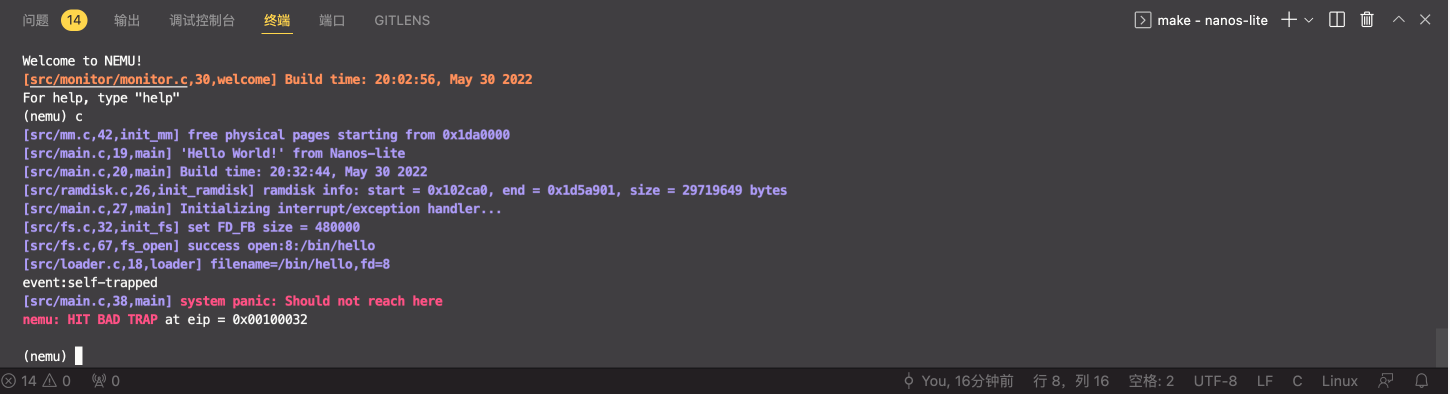
\includegraphics[scale = 0.53]{./img/9.png}
\end{center}

\subsection{实现上下文切换}
根据实验指导书的要求,我们需要在这部分实现如下内容:
\begin{itemize}
\item PTE 的\_umake()函数;
\item Nanos-lite的schedule()函数;
\item 修改 ASYE 中 asm\_trap()的实现,使得从 irq\_handle()返回后,先将栈顶指针切换到新进程的陷阱帧,然后才根据陷阱帧的内容恢复现场,从而完成上下文切换的本质操作。
\end{itemize}
在nexus-am/am/arch/x86-nemu/src/pte.c中完成\_umake()函数。这个函数在加载程序时完成上下文的创建,在这里,我们依次把入口的三个参数和指令寄存器入栈,然后按PA3实现过的思路,完成对tf内容的初始化设置。
\begin{lstlisting}[language = C++]
_RegSet *_umake(_Protect *p, _Area ustack, _Area kstack, void *entry, char *const argv[], char *const envp[]) {
  extern void* memcpy(void *, const void *, int);
  int arg1 = 0;
  char *arg2 = NULL;
  memcpy((void*)ustack.end - 4, (void*)arg2, 4);
  memcpy((void*)ustack.end - 8, (void*)arg2, 4);
  memcpy((void*)ustack.end - 12, (void*)arg1, 4);
  memcpy((void*)ustack.end - 16, (void*)arg1, 4);

  _RegSet tf;
  tf.eflags = 0x02 | FL_IF;
  tf.cs = 0;
  tf.eip = (uintptr_t) entry;
  void *ptf = (void*) (ustack.end - 16 - sizeof(_RegSet));
  memcpy(ptf, (void*)&tf, sizeof(_RegSet));
  return (_RegSet*) ptf;
}
\end{lstlisting}
在nanos-lite/src/proc.c中,完成schedule()函数,用于返回现场。
\begin{lstlisting}[language = C++]
_RegSet* schedule(_RegSet *prev) {
  if(current != NULL) {
    current -> tf = prev;
  }
  current = pcb[0];
  Log("ptr = 0x%x\n", (uint32_t)current -> as.ptr);
  _switch(&current -> as);
  return current -> tf;
}

\end{lstlisting}
然后在nanos-lite/src/irq.c中,完善对\_EVENT\_TRAP 事件的处理。也就是,Nanos-lite 收到\_EVENT\_TRAP 事件后,调用 schedule()并返回其现场。

\begin{lstlisting}[language = C++]
static _RegSet* do_event(_Event e, _RegSet* r) {
  switch (e.event) {
    case _EVENT_SYSCALL:
      return do_syscall(r);
    case _EVENT_TRAP:
      printf("event:self-trapped\n");
      return schedule(r);
    default: 
      panic("Unhandled event ID = %d", e.event);
  }

  return NULL;
}
\end{lstlisting}

最后,修改nexus-am/am/arch/x86-nemu/src/trap.S中asm\_trap()的实现:从中断控制函数返回后,先把栈顶指针切换到新进程的trap帧,再据此恢复现场。
\begin{lstlisting}[language=C++]
asm_trap:
  pushal

  pushl %esp
  call irq_handle

  # addl $4, %esp
  movl %eax, %esp

  popal
  addl $8, %esp

  iret
\end{lstlisting}
于是我们可以通过自陷的方式触发仙剑奇侠传程序了。
\begin{center}
  \includegraphics*[scale = 0.35]{img/10}
\end{center}

\subsection{分时多任务}
我们已经实现了分页和上下文切换,实际上已经可以支持多任务分时运行了。这部分我们需要做的就是完善调度机制,让仙剑奇侠传和其他程序切换运行。
首先修改nanos-lite/src/main.c当中加载程序的代码,把待运行的程序都载入。
\begin{lstlisting}[language = C++]
load_prog("/bin/pal");
load_prog("/bin/hello");
\end{lstlisting}
接着修改nanos-lite/src/proc.c中调度的代码,让 schedule()轮流返回仙剑奇侠传和 hello 的现场。这里只要按指导书所说,修改current的值即可。
\begin{lstlisting}[language = C++]
_RegSet* schedule(_RegSet *prev) {
  if(current != NULL) {
    current -> tf = prev;
  }
  current = (current == &pcb[0]? &pcb[1] : &pcb[0]);
  Log("ptr = 0x%x\n", (uint32_t)current -> as.ptr);
  _switch(&current -> as);
  return current -> tf;
}
\end{lstlisting}
最后,修改nanos-lite/src/irq.c当中do\_event() 的代码,在处理完syscall之后,调用 schedule()函数并返回其现场
\begin{lstlisting}[language=C++]
static _RegSet* do_event(_Event e, _RegSet* r) {
  switch (e.event) {
    case _EVENT_SYSCALL:
      // return do_syscall(r);
      do_syscall(r);
      return schedule(r);
    case _EVENT_TRAP:
      printf("event:self-trapped\n");
      return schedule(r);
    default: 
      panic("Unhandled event ID = %d", e.event);
  }

  return NULL;
}
\end{lstlisting}
于是,我们完成了hello和仙剑奇侠传的分时运行。
\begin{center}
  \includegraphics*[scale = 0.35]{img/11}
\end{center}

\subsection{优先级调度}
实现两个程序分时运行之后,仙剑奇侠传的运行速度有了明显的下降,于是我们在这部分对调度频率比例进行修改,让仙剑奇侠传能更多地占用处理器资源,运行得稍快些。需要修改的依然是nanos-lite/src/proc.c文件的schedule()代码,设置frequency为频率比例,num为当前程序运行次数,仙剑奇侠传运行frequency次,才切换到hello程序运行一次,并重新计数。
\begin{lstlisting}[language = C++]
_RegSet* schedule(_RegSet *prev) {
  if(current != NULL) {
    current -> tf = prev;
  }
  else {
    current = &pcb[current_game];
  }
  static int num = 0;
  static const int frequency = 1000;
  if(current == &pcb[current_game]) {
    num++;
  }
  else {
    current = &pcb[current_game];
  }
  if(num == frequency) {
    current = &pcb[1];
    num = 0;
  }
  // current = (current == &pcb[0]? &pcb[1] : &pcb[0]);
  // Log("ptr = 0x%x\n", (uint32_t)current -> as.ptr);
  _switch(&current -> as);
  return current -> tf;
}
\end{lstlisting}
实现了指定频率比例的优先级调度之后,仙剑奇侠传的运行速度得到了提升。
\begin{center}
  \includegraphics*[scale = 0.3]{img/12}
\end{center}

\section{阶段三: 时钟中断与其他}
\subsection{时钟中断}
如果程序陷入了死循环,或程序是一个高占用的有害程序,系统应当能提供一些机制来强制将它结束。这就是系统设定的硬件中断。在我们的实验中只实现时钟中断这一种即可,这就是本阶段的任务。根据指导书,首先,在 nemu/include/cpu/reg.h的cpu 结构体中添加一个 bool 成员 INTR
\begin{lstlisting}[language = C++]
bool INTR;
\end{lstlisting}
然后在nemu/src/cpu/intr.c 的dev\_raise\_intr()中将 INTR 引脚设置为高电平。
\begin{lstlisting}[language = C++]
void dev_raise_intr() {
  cpu.INTR = true;
}
\end{lstlisting}
在nemu/src/cpu/exec/exec.c文件的exec\_wrapper()函数末尾添加轮询 INTR 引脚的代码。其具体功能是,每次执行完一条指令就查看是否有硬件中断到来,具体代码在指导书中已经直接给出。
\begin{lstlisting}[language = C++]
#define TIME_IRQ 32

  if(cpu.INTR & cpu.eflags.IF) {
    cpu.INTR = false;
    extern void raise_intr(uint8_t NO, vaddr_t ret_addr);
    raise_intr(TIME_IRQ, cpu.eip);
    update_eip();
  }
\end{lstlisting}

然后修改 nemu/src/cpu/intr.c当中raise\_intr()的代码

\begin{lstlisting}[language = C++]
memcpy(&t1, &cpu.eflags, sizeof(cpu.eflags));
rtl_li(&t0, t1);
rtl_push(&t0);
cpu.eflags.IF = 0;
rtl_push(&cpu.cs);
rtl_li(&t0, ret_addr);
rtl_push(&t0);
\end{lstlisting}
这部分代码使得程序在保存 EFLAGS 寄存器后,将其IF位设为 0,让处理器进入关中断的状态。这几部分代码完成了时钟中断的硬件操作,还需要在ASYE添加对时钟中断的支持,完成软件层面的系统中断实现。

首先在nexus-am/am/arch/x86-nemu/src/asye.c声明vectime()作为时钟中断的入口函数,然后在asye\_init()中添加int 32的门描述符。

\begin{lstlisting}[language = C++]
idt[32] = GATE(STS_TG32, KSEL(SEG_KCODE), vectime, DPL_USER);
\end{lstlisting}
在irq\_handle()函数中添加\_EVENT\_IRQ\_TIME事件。
\begin{lstlisting}[language = C++]
_RegSet* irq_handle(_RegSet *tf) {
  _RegSet *next = tf;
  if (H) {
    _Event ev;
    switch (tf->irq) {
      case 0x80: 
        ev.event = _EVENT_SYSCALL; 
        break;
      case 0x81:
        ev.event = _EVENT_TRAP;
        break;
      case 32:
        ev.event = _EVENT_IRQ_TIME;
        break;
      default: 
        ev.event = _EVENT_ERROR; 
        break;
    }

    next = H(ev, tf);
    if (next == NULL) {
      next = tf;
    }
  }

  return next;
}
\end{lstlisting}
然后,在nanos-lite/src/irq.c当中,为do\_event() 函数添加\_EVENT\_IRQ\_TIME事件的操作。
\begin{lstlisting}[language = C++]
static _RegSet* do_event(_Event e, _RegSet* r) {
  switch (e.event) {
    case _EVENT_SYSCALL:
      // return do_syscall(r);
      do_syscall(r);
      return schedule(r);
    case _EVENT_TRAP:
      printf("event:self-trapped\n");
      return schedule(r);
    case _EVENT_IRQ_TIME: 
      Log("event:IRQ_TIME");
      return schedule(r);
    default: 
      panic("Unhandled event ID = %d", e.event);
  }

  return NULL;
}
\end{lstlisting}
即,收到时钟中断的信号后,直接调用schedule()函数进行调度,并输出一个时钟中断的调度信息,以便我们验证程序结果。

还需要在nexus-am/am/arch/x86-nemu/src/trap.S中对vectime函数进行注册。
\begin{lstlisting}[]
.globl vectime; vectime: pushl $0; pushl $32; jmp asm_trap 
\end{lstlisting}


最后,为了保证处理器运行程序时能对时钟中断做出正确响应,还要修改nexus-am/am/arch
/x86¬nemu/src/pte.c中的\_umake()函数,对eflags寄存器进行对应的设置。
\begin{lstlisting}[language = C++]
_RegSet *_umake(_Protect *p, _Area ustack, _Area kstack, void *entry, char *const argv[], char *const envp[]) {
  extern void* memcpy(void *, const void *, int);
  int arg1 = 0;
  char *arg2 = NULL;
  memcpy((void*)ustack.end - 4, (void*)arg2, 4);
  memcpy((void*)ustack.end - 8, (void*)arg2, 4);
  memcpy((void*)ustack.end - 12, (void*)arg1, 4);
  memcpy((void*)ustack.end - 16, (void*)arg1, 4);

  _RegSet tf;
  tf.eflags = 0x02 | FL_IF;
  tf.cs = 0;
  tf.eip = (uintptr_t) entry;
  void *ptf = (void*) (ustack.end - 16 - sizeof(_RegSet));
  memcpy(ptf, (void*)&tf, sizeof(_RegSet));
  return (_RegSet*) ptf;
}
\end{lstlisting}
时钟中断成功实现。
\begin{center}
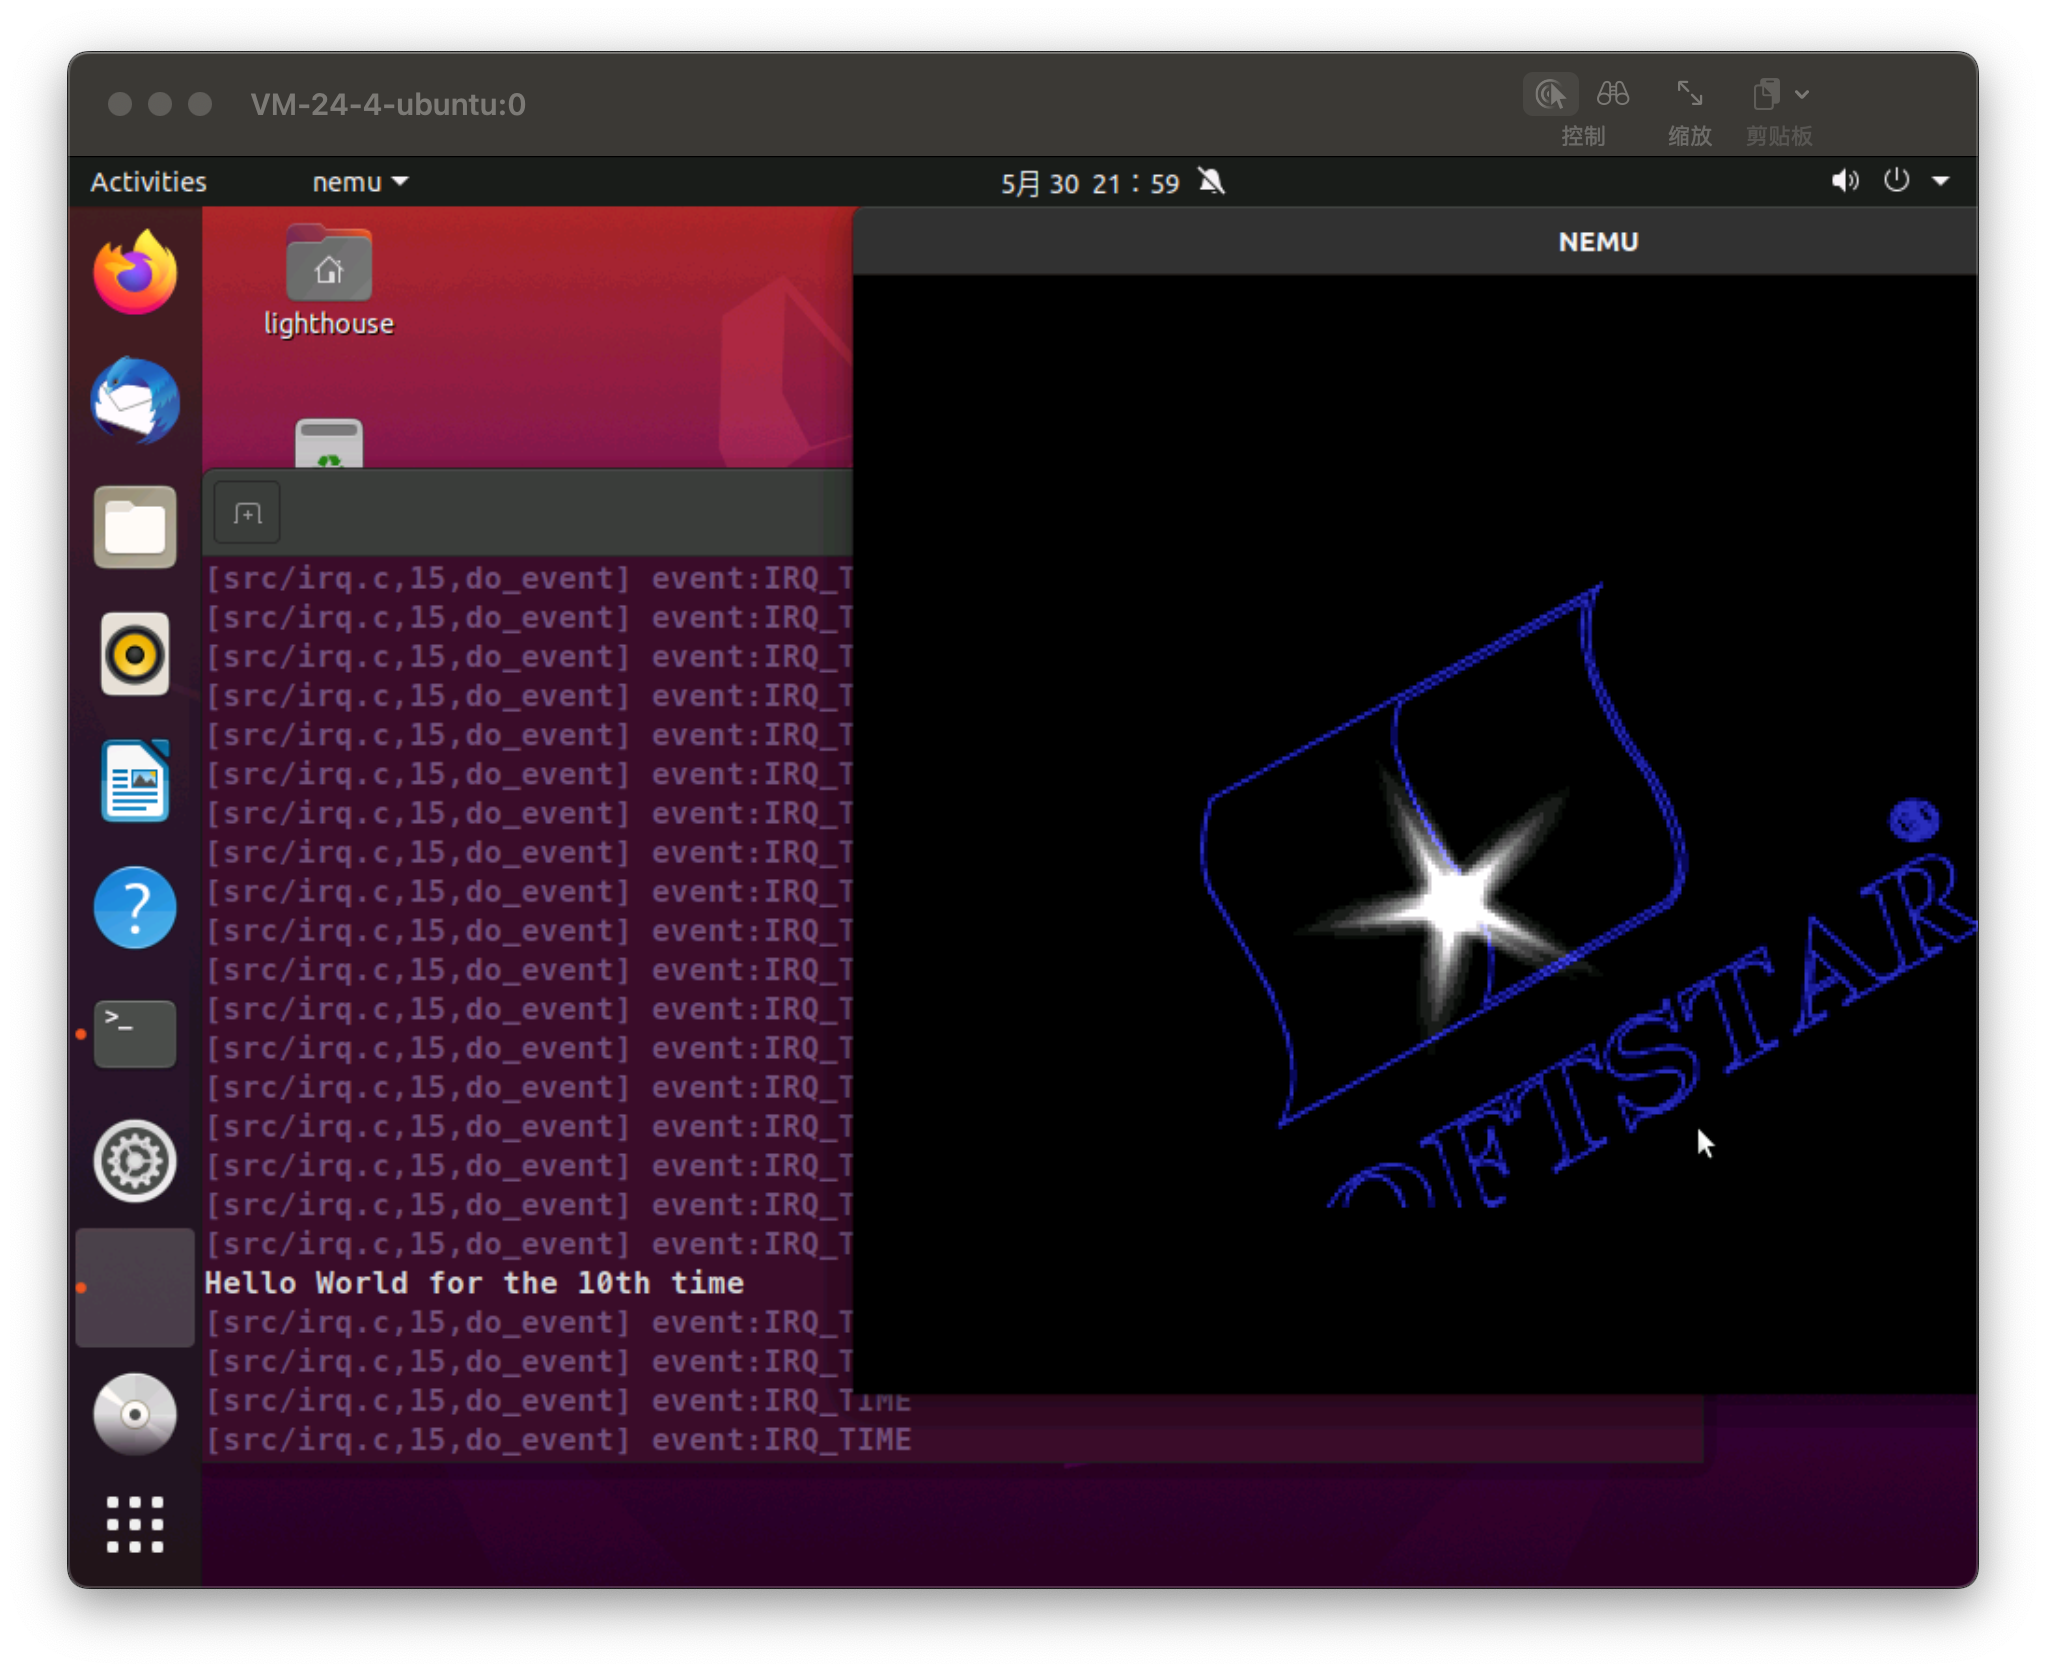
\includegraphics[width=0.9\textwidth]{img/13.png}
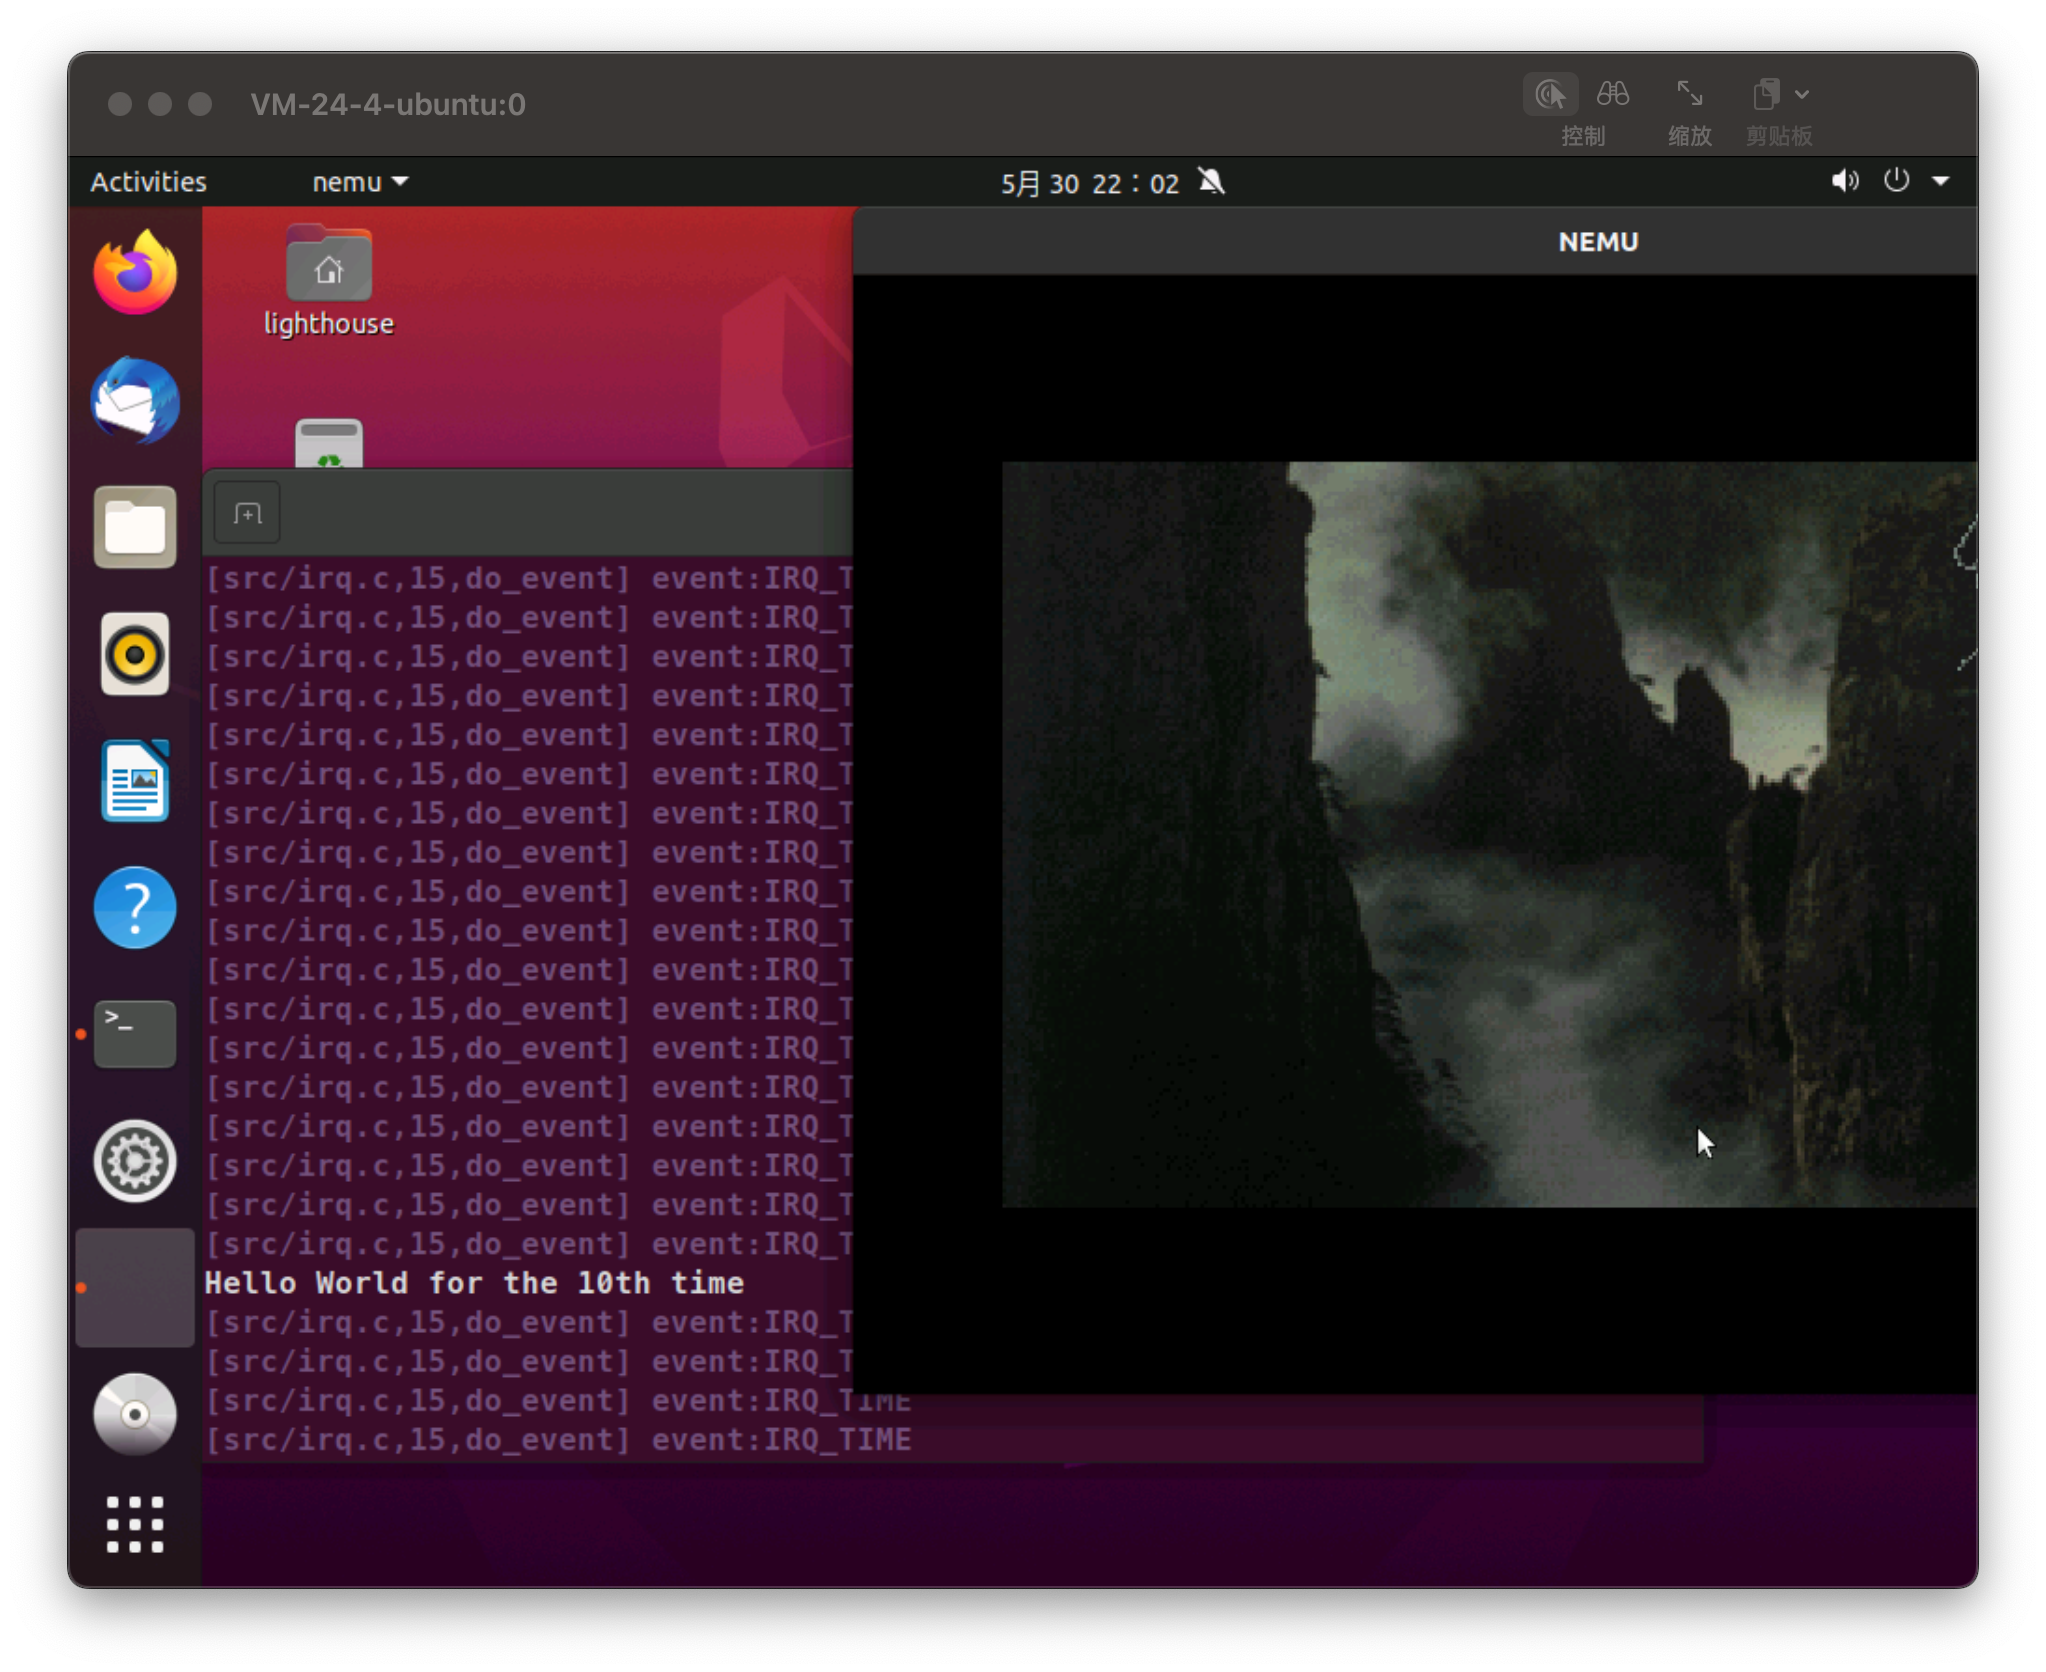
\includegraphics[width=0.9\textwidth]{img/14.png}
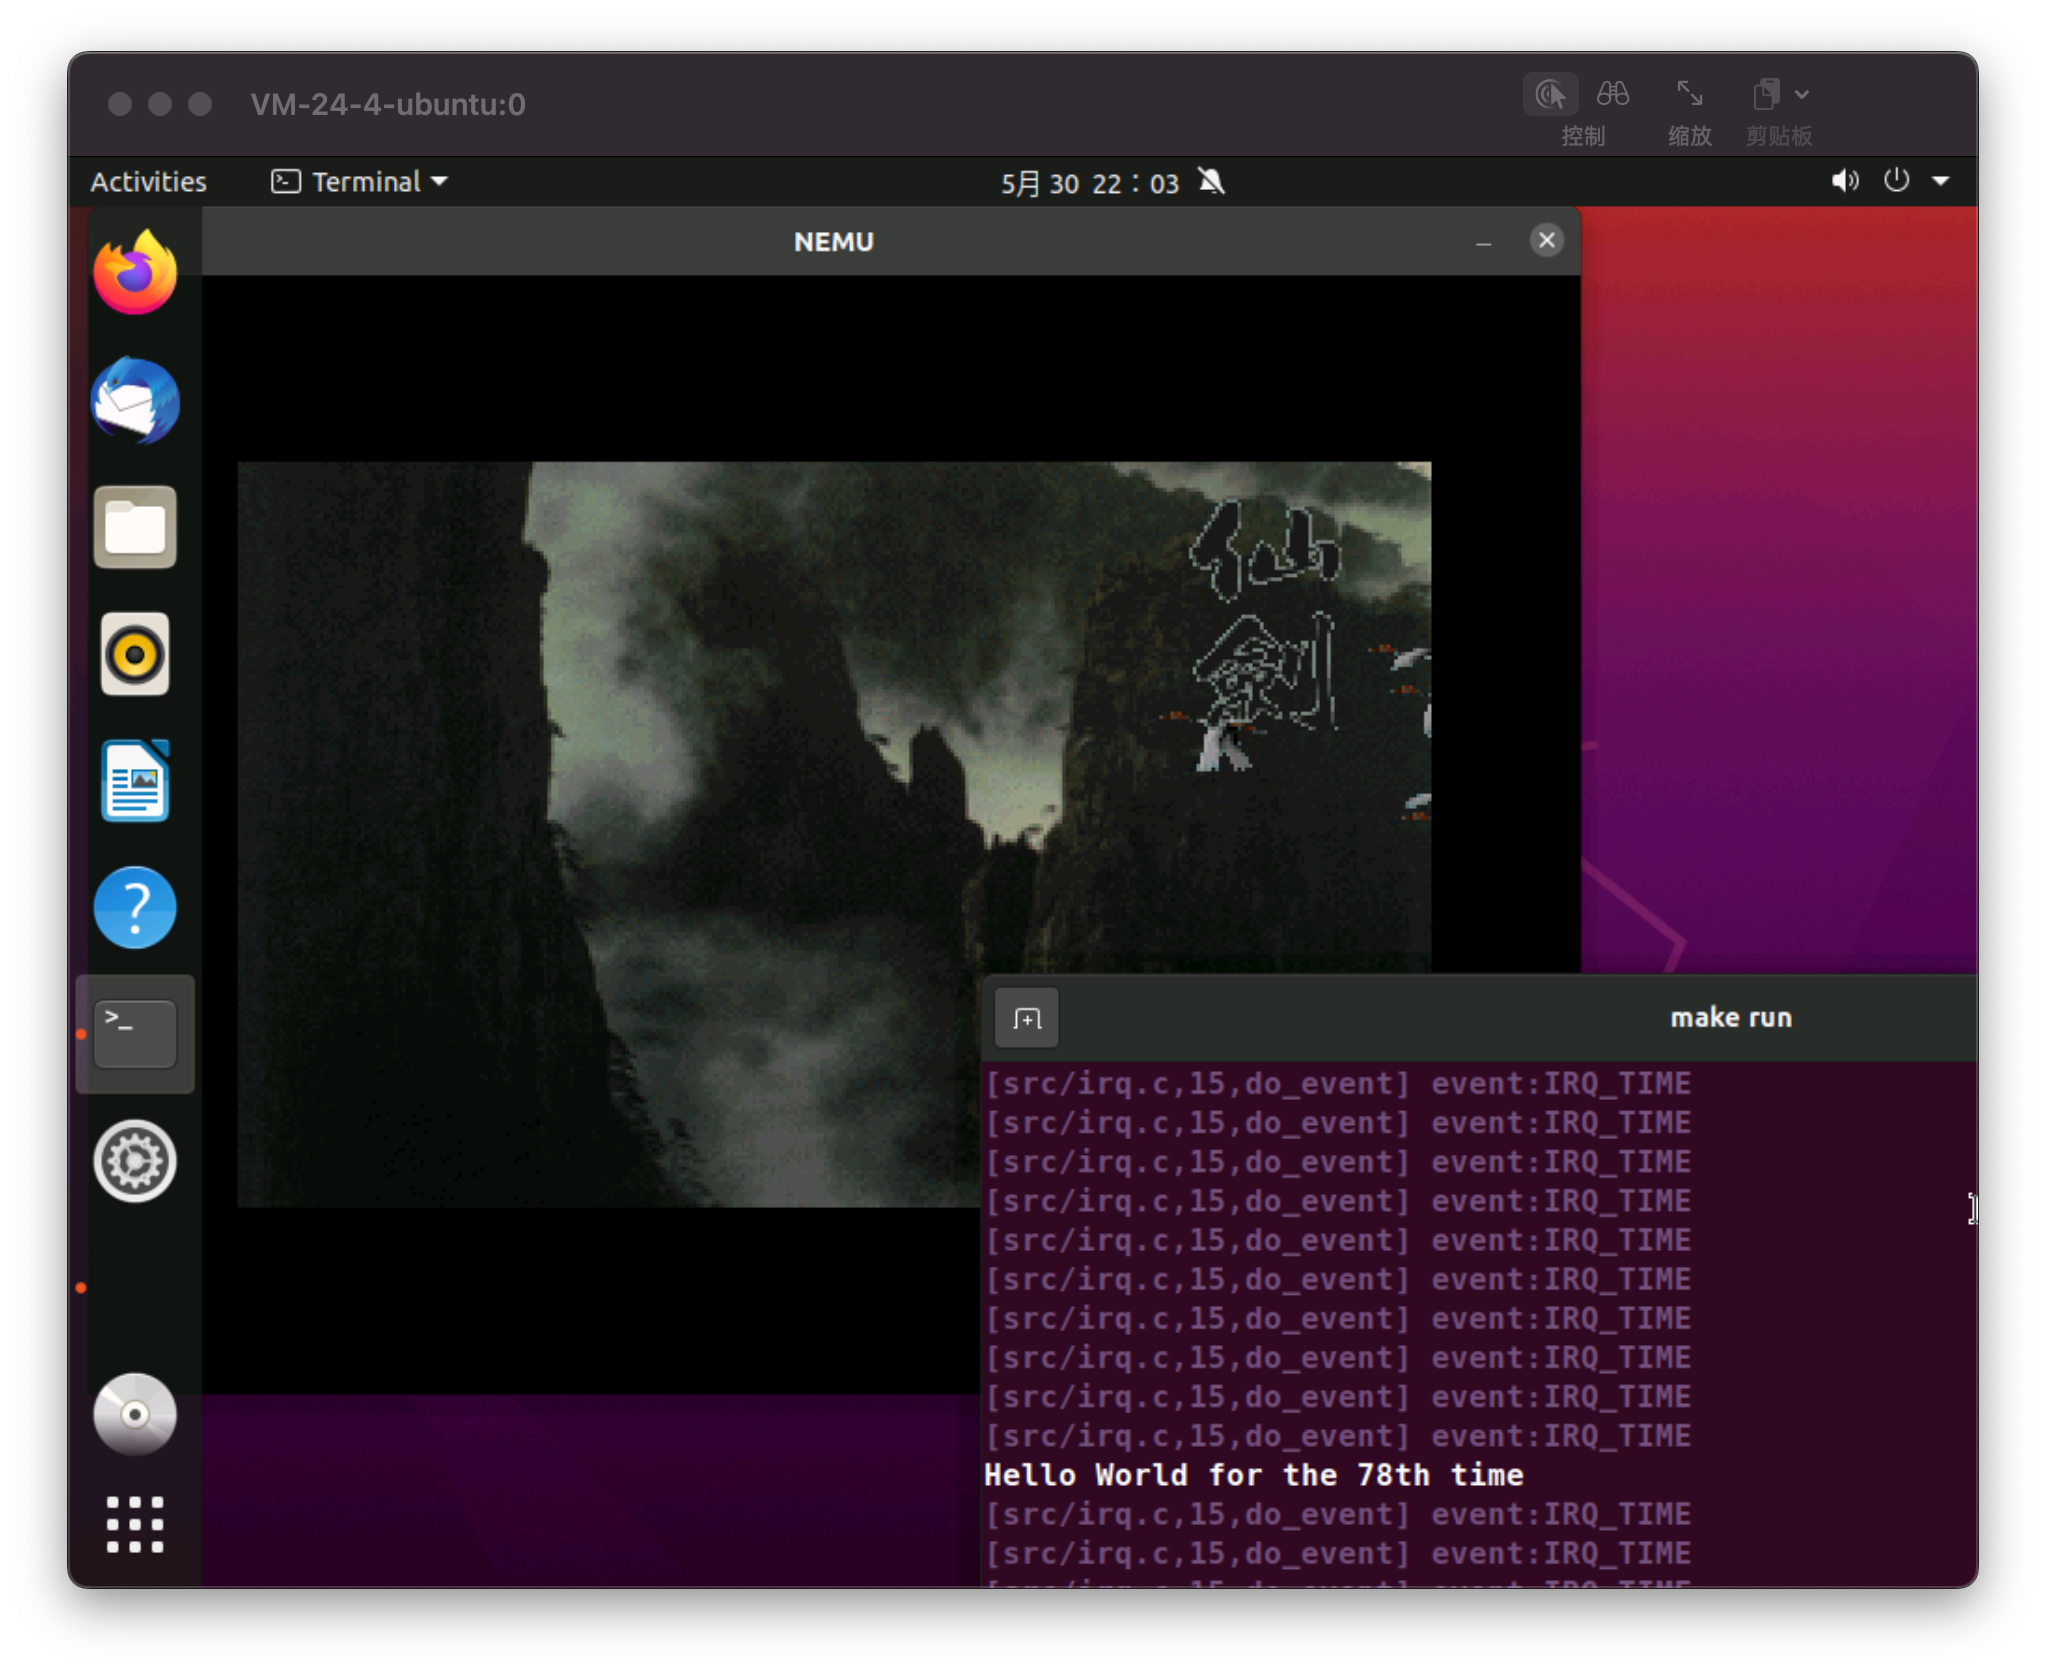
\includegraphics[width=0.9\textwidth]{img/15.png}
\end{center}

\subsection{展示计算机系统}
这部分为系统添加按键功能,当用户按下F12的时候,让游戏在仙剑奇侠传和videotest之间切换。首先在nanos-lite/src/proc.c的schedule()函数中,通过一个变量 current\_game 来记录当前的游戏,在current\_game和hello程序之间进行调度。通过编写switch\_current\_game()函数,在游戏之间进行切换。
\begin{lstlisting}[language = C++]
int current_game = 0;
void switch_current_game() {
  current_game = 2 - current_game;
  Log("current_game = %d", current_game);
}
\end{lstlisting}
在nanos-lite/src/device.c的events\_read()函数中,添加对按键F12的检测和响应处理
\begin{lstlisting}[language = C++]
if(down && key == _KEY_F12) {
  extern void switch_current_game();
  switch_current_game();
  Log("key down:_KEY_F12, switch current game0!");
}
\end{lstlisting}
于是,程序按照我们的设计,最初是仙剑奇侠传和 hello 程序分时运行,按下 F12 之后,就变成 videotest 和 hello 程序分时运行。
\begin{center}
  \includegraphics*[scale=0.35]{img/16.png}
\end{center}


\end{document}
